% Epstein: Why Is Forgetting Important?
% Virtual Memory for Transformer Context Windows
% Target: SOSP 2026 — acmart sigplan format

\documentclass[sigplan,screen,anonymous]{acmart}

% Anonymous submission
\settopmatter{printacmref=false}
\renewcommand\footnotetextcopyrightpermission[1]{}
\pagestyle{plain}

\usepackage{booktabs}
\usepackage{subcaption}
\usepackage{tikz}
\usetikzlibrary{arrows.meta,positioning,fit,backgrounds,decorations.pathreplacing}

\begin{document}

\title{Epstein: Why Is Forgetting Important?}
\subtitle{Virtual Memory for Transformer Context Windows}

\author{Anonymous}
\affiliation{\institution{Anonymous}}

\begin{abstract}
Transformer context windows are managed as fixed-size append-only
buffers. When the buffer fills, systems either discard the
conversation, summarize it lossily, or demand a larger window---the
equivalent of buying more RAM rather than implementing virtual memory.
We find this analogy is not merely illustrative but architectural:
context windows are L1 caches that need a memory hierarchy, not bigger
caches.

We present Tinkuy, a virtual memory system for transformer context
windows. The system introduces \emph{cooperative paging}, in which the
model participates in its own memory management by producing structured
tensor summaries with declared losses before eviction. Tensor
compression is stable over 60+ turns at 97.3\% compression ratio---the
model converges on appropriate summaries without divergence. An
episodic page table tracks present and evicted content, enabling
demand paging at retrieval time.

Our key finding is that managed forgetting requires preserving
\emph{provenance}, not just conclusions. We define three drift
dimensions---Factual Retention, Coherence Retention, and Working Set
trajectory---and show that existing approaches collapse to compaction:
high FR, zero CR. Arbitrary rationale details vanish within 30 turns
even when physically present in context. A dependency edge protocol
captures reasoning chains at decision time; a provenance page fault
mechanism reconstructs chains on demand. Active provenance recovery
achieves 2/2 on root-cause probes where passive CR scores 0/8.

We validate the system on AI coding agent workloads. A live session
achieves 95\% cache hit rate with the projective gateway managing a
20K token projection from 98K tokens of raw conversation. Episodic
page tables reduce token consumption by 68\% while preserving
retrieval quality; flat page tables cause catastrophic 38$\times$
amplification. The interface between the VM and the model is not
neutral---it changes the model's access pattern, an effect with no
analog in hardware VM.
\end{abstract}

\maketitle

%% ============================================================
%% 1. INTRODUCTION
%% ============================================================

\section{Introduction}

Consider a worker who can only use one desk. Everything the worker
needs---instructions, reference documents, notes from every
conversation, results of every task---must fit on that desk. If it is
not on the desk, it does not exist. The worker's assistant prepares
the desk before each task, diligently piling on the full employee
handbook (even when only one chapter is needed), three copies of the
office directory (filed under different names), and every memo from
every previous task---including ones the worker has already read and
acted on. The assistant never removes anything.

When the desk overflows, one of two things happens. A supervisor
sweeps half the desk into the trash, leaving a short note: ``you were
working on something, here's a summary.'' Or the desk simply cannot
accept new work, and the worker stops. Everyone's solution is to buy a
bigger desk. The vendors obliged: desks five times larger, ten times
larger, fifty times larger. But the assistant's behavior does not
change. Bigger desks fill up too, just slower and more expensively.
And the worker actually performs worse at very large desks---too much
clutter to find what matters.

This is the state of context window management in large language
models. The desk is the context window. The assistant is the client
application that assembles the message array. The supervisor is lossy
summarization. The bigger desk is the 200K, 1M, 2M token window. An
empirical analysis of 857 coding agent sessions consuming 4.45 billion
tokens reveals 21.8\% structural waste---content that consumes
attention without contributing to the task. The waste scales linearly
with desk size.

The worker does not need a bigger desk. The worker needs a library.

In 1961, the Atlas computer introduced demand
paging~\cite{kilburn1962atlas}---the architectural insight that a
program's working memory need not be physically resident, so long as
it can be brought in on demand. Before Atlas, programmers managed
overlays manually, partitioning programs into segments and tracking
what was loaded. Virtual memory made this unnecessary. We argue that
the same architectural insight applies to transformer context windows:
they are L1 caches that need a memory hierarchy, not bigger caches.

This paper presents Tinkuy, a virtual memory system for transformer
context windows. The filing clerk sits between the client and the
model: before each turn, it files away old content (leaving a
forwarding note in a \emph{page table}), and when the model needs
something that was filed, it pulls it back instantly. The model reads
the notes and understands them---it requests recalls without being
told the system exists. When a document keeps getting filed and
immediately requested back, the system pins it: ``you always need this
one.'' Every filed item carries an honest note about what was lost in
the filing.

The architecture was invented sixty years ago. It was just in a
building across campus that nobody in AI had visited.

The system makes five contributions:

\begin{enumerate}
\item \textbf{Empirical evidence that context management is VM.} We
  characterize waste in 857 production sessions, showing that context
  windows suffer from the same fragmentation and duplication that
  motivated virtual memory in hardware (\S\ref{sec:problem}).

\item \textbf{The inverted cost model.} In hardware VM, keeping pages
  in memory is cheap and faulting is expensive. In transformer VM,
  keeping is expensive ($O(n^2)$ attention) and faulting is cheap (one
  API round trip). This inverts the optimization objective from
  ``minimize faults'' to ``minimize total cost''
  (\S\ref{sec:cost-model}).

\item \textbf{Cooperative memory management.} The model participates
  in its own eviction by producing structured tensor summaries with
  declared information losses. Tensor compression is stable over 60+
  turns---the model converges on an appropriate compression ratio
  without divergence (\S\ref{sec:tensors}).

\item \textbf{Episodic page tables.} The page table interface changes
  the model's access pattern---an effect with no analog in hardware VM
  where the page table is invisible to the application. Flat page
  tables cause 38$\times$ token amplification; episodic coalescing
  reduces overhead to 0.94$\times$ baseline
  (\S\ref{sec:episodic-pt}).

\item \textbf{Provenance edges that break the attention ceiling.}
  Passive coherence retention decays to 0/8 on arbitrary rationale
  details by turn 29. Active provenance recovery via dependency edges
  and trace signals achieves 2/2---exceeding the limit set by the
  model's natural attention (\S\ref{sec:cr-eval}).
\end{enumerate}

%% ============================================================
%% 2. THE PROBLEM
%% ============================================================

\section{The Problem: Context Windows as Mismanaged Memory}
\label{sec:problem}

\subsection{Empirical Waste Characterization}

We analyzed 857 Claude Code sessions comprising 4.45 billion tokens of
API traffic. These sessions represent production AI coding agent
workloads: multi-turn conversations with extensive tool use (file
reads, edits, shell commands) interleaved with reasoning.

Structural waste---content that consumes attention cost without
contributing to the current task---accounts for 21.8\% of all tokens
processed. The waste taxonomy breaks down as follows:

\begin{itemize}
\item \textbf{Tool schemas (11.0\%):} Complete tool definitions
  re-sent on every API call. These are static across the session and
  identical across sessions, yet consume attention on every turn.

\item \textbf{Stale results (8.7\%):} Tool results from earlier turns
  that have been superseded by subsequent actions. A file read from
  turn 3 that was overwritten by an edit on turn 7 still occupies
  context on turn 15.

\item \textbf{Duplication (2.2\%):} Repeated content from
  re-reads of the same files, repeated instructions, and
  conversation patterns that echo earlier statements.
\end{itemize}

This waste scales linearly with context window size. A 200K token
window wastes approximately 43K tokens. A hypothetical 1M token window
would waste approximately 218K tokens. The problem is not capacity
but management.

\subsection{The Inverted Cost Model}
\label{sec:cost-model}

In hardware virtual memory, the cost structure is:
\begin{itemize}
\item \textbf{Keeping a page resident:} Essentially free. A page in
  RAM consumes physical memory but no computation per access cycle.
\item \textbf{Page fault:} Expensive. Disk access takes
  $10^4$--$10^6\times$ longer than memory access.
\end{itemize}

This cost structure makes the optimization objective clear: minimize
page faults. Belady's optimal algorithm~\cite{belady1966anomaly}, LRU,
and their approximations all pursue this objective.

Transformer context windows invert this structure:
\begin{itemize}
\item \textbf{Keeping content in context:} Expensive. Each token in
  context participates in $O(n^2)$ attention computation on every
  forward pass. Keeping a stale 5,000-token tool result costs
  attention on every subsequent turn.
\item \textbf{Page fault:} Cheap. Retrieving evicted content requires
  one additional API round trip---latency measured in seconds, cost
  measured in output tokens for the request.
\end{itemize}

This inversion changes the optimal policy. In hardware VM, aggressive
eviction is dangerous (faults are expensive). In transformer VM,
aggressive eviction is correct by default (keeping is expensive).
FIFO---the simplest possible policy, generally considered poor for
hardware VM---performs surprisingly well because it systematically
removes the oldest content, and older content is precisely what
contributes most to cumulative attention waste.

The exception is \emph{provenance}: the reasoning chain that connects
decisions to their rationale. Provenance content is small (a few
hundred tokens per decision) but irreplaceable---once the ``why''
behind a decision is evicted without a forwarding pointer, no amount
of re-reading source material will reconstruct it. This creates a
bimodal eviction policy: aggressive for bulk content, protective for
provenance.

\subsection{Why Bigger Windows Don't Solve It}

The industry response to context limitations has been larger
windows---from 4K to 8K to 32K to 128K to 200K to 1M tokens.
This is the equivalent of buying more RAM rather than implementing
virtual memory.

Larger windows do not address the structural waste identified in
\S\ref{sec:problem}. Tool schemas still consume 11\% of a 1M window.
Stale results still accumulate. The $O(n^2)$ attention cost increases
with window size, making the waste more expensive, not less. And the
fundamental problem remains: when the window fills---and it always
fills eventually---there is no hierarchy to fall back on.

Virtual memory solved this problem for hardware in 1961. We argue
the same architectural insight applies to transformer context windows.

%% ============================================================
%% 3. SYSTEM DESIGN
%% ============================================================

\section{System Design}

\subsection{Three Generations of Architecture}

Tinkuy is the third iteration of a virtual memory system for
transformer context windows, following two earlier systems that
informed its design through their failures.

\paragraph{Pichay (transparent proxy).}
The first system was an HTTP proxy that intercepted API calls between
the client (an AI coding agent) and the model provider. The proxy
modified the client's message array---injecting page tables, removing
evicted content, inserting tensor summaries. This architecture failed
in four successive iterations due to what we term \emph{proxy
gravity}: the persistent pull toward passing through the client's
message array with minimal modification, rather than constructing the
correct payload from first principles.

The fundamental problem is ownership. In a proxy architecture, the
client owns the conversation---the proxy borrows it, modifies it, and
returns it. Every modification must be compatible with the client's
assumptions about what it sent. When the proxy removes a tool result
the client expects to be present, or reorders messages for cache
optimization, the client's assumptions break.

\paragraph{Hamut'ay (cooperative projector).}
The second system introduced the key innovation that survives into
Tinkuy: \emph{cooperative eviction}. Rather than evicting content
unilaterally, the system asks the model to produce a tensor---a
structured summary with explicitly declared information losses---before
removing the original. This transforms eviction from a destructive
operation into a collaborative compression.

Hamut'ay demonstrated that the model is a capable memory curator. In
backtesting (replaying four completed conversations through the
projector), tensor compression achieved 97.3\% reduction across 159KB
of original content. More significantly, in a sustained live chat
session exceeding 60 turns, tensor size remained stable---the model
converges on an appropriate compression ratio without producing
progressively larger or smaller summaries. However, Hamut'ay was still
architecturally a proxy. It suffered from the same ownership problem,
though the cooperative protocol masked some of its symptoms.

\paragraph{Tinkuy (projective gateway).}
The current system resolves the ownership problem by eliminating the
proxy pattern entirely. Tinkuy maintains a \emph{projection}---an
internal representation of the conversation state---and synthesizes
API payloads from this projection. The client's original message array
is ingested on arrival and decomposed into content blocks, but the API
payload sent to the model provider is constructed from the projection,
not modified from the client's input.

This is the ``gateway owns the conversation'' principle. The client
sends messages; the gateway decides what the model sees. This
eliminates proxy gravity because there is no client payload to
gravitationally attract minimal modifications.

\subsection{The Price of Ownership}
\label{sec:price}

The projective gateway is architecturally correct but engineering-hard.
When the client owns the message array, it naturally satisfies the
API's layout constraints---the constraints are implicit in how clients
construct messages. When the gateway synthesizes payloads from a
projection, every constraint must be explicitly enforced:

\begin{itemize}
\item \textbf{Alternation:} The Anthropic Messages API requires strict
  user/assistant message alternation. Eviction can remove messages that
  were providing alternation padding.

\item \textbf{Tool pairing:} Every \texttt{tool\_use} block in an
  assistant message must have a matching \texttt{tool\_result} in the
  next user message, and vice versa. Eviction can orphan either side
  of a pair.

\item \textbf{Content block ordering:} In user messages that follow
  tool use, \texttt{tool\_result} blocks must precede text blocks.
  Region merging during synthesis can violate this ordering.

\item \textbf{Content sanitization:} Each content block type permits
  only specific fields. Internal metadata must be stripped before the
  payload reaches the API.
\end{itemize}

These constraints are undocumented in the API specification and were
discovered empirically through error responses. A pre-flight
validator catches violations before they reach the API. A tool
pairing repair pass strips orphaned blocks created by eviction. These
are not research contributions---they are the cost of the
abstraction. We report them because they determine whether the
architecture is practical, not just correct.

\subsection{Five-Region Projection}
\label{sec:regions}

\begin{figure}[t]
\centering
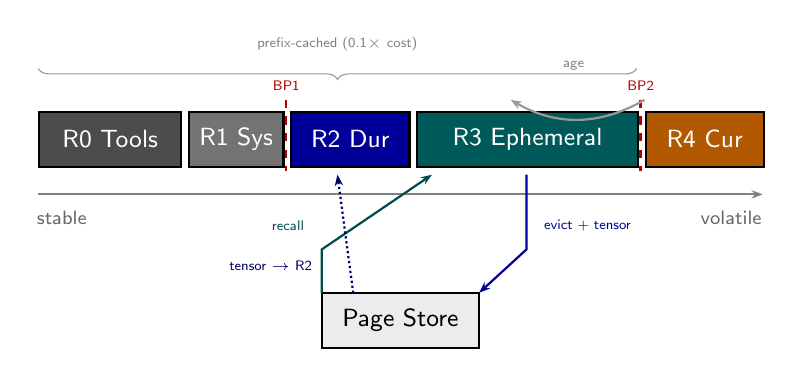
\begin{tikzpicture}[
  region/.style={
    draw, thick, minimum height=0.7cm, text=white, font=\small\sffamily,
    anchor=west,
  },
  label/.style={font=\scriptsize\sffamily, anchor=west},
  arrow/.style={-{Stealth[length=4pt]}, thick},
  brace/.style={decorate, decoration={brace, amplitude=4pt, mirror}},
]

% Region bars — widths proportional to typical token share
\node[region, fill=black!70, minimum width=1.8cm] (r0) at (0,0) {R0 Tools};
\node[region, fill=black!55, minimum width=1.2cm] (r1) at (1.9,0) {R1 Sys};
\node[region, fill=blue!60!black, minimum width=1.5cm] (r2) at (3.2,0) {R2 Dur};
\node[region, fill=teal!70!black, minimum width=2.8cm] (r3) at (4.8,0) {R3 Ephemeral};
\node[region, fill=orange!70!black, minimum width=1.5cm] (r4) at (7.7,0) {R4 Cur};

% Stability gradient arrow beneath
\draw[arrow, black!50] (0, -0.7) -- (9.2, -0.7);
\node[font=\scriptsize\sffamily, black!60] at (0.3, -1.0) {stable};
\node[font=\scriptsize\sffamily, black!60] at (8.8, -1.0) {volatile};

% Cache breakpoints — dashed lines above
\draw[dashed, red!70!black, thick] (3.15, 0.5) -- (3.15, -0.4);
\node[font=\tiny\sffamily, red!70!black, anchor=south] at (3.15, 0.5) {BP1};

\draw[dashed, red!70!black, thick] (7.65, 0.5) -- (7.65, -0.4);
\node[font=\tiny\sffamily, red!70!black, anchor=south] at (7.65, 0.5) {BP2};

% Page Store — external box
\node[draw, thick, fill=gray!15, minimum width=2.0cm, minimum height=0.7cm,
      font=\small\sffamily] (store) at (4.6, -2.3) {Page Store};

% Evict arrow: R3 → down to store, with tensor label
\draw[arrow, blue!60!black] (6.2, -0.45) -- (6.2, -1.4) -- (5.6, -1.95);
\node[font=\tiny\sffamily, blue!60!black, anchor=west] at (6.3, -1.1) {evict + tensor};

% Recall arrow: store → up to R3
\draw[arrow, teal!60!black] (3.6, -1.95) -- (3.6, -1.4) -- (5.0, -0.45);
\node[font=\tiny\sffamily, teal!60!black, anchor=east] at (3.5, -1.1) {recall};

% Tensor promotion: store → R2
\draw[arrow, blue!40!black, densely dotted] (4.0, -1.95) -- (3.8, -0.45);
\node[font=\tiny\sffamily, blue!40!black, anchor=east] at (3.6, -1.6) {tensor $\to$ R2};

% Aging arrow: R4 → R3
\draw[arrow, black!40] (7.7, 0.5) to[bend left=30] (6.0, 0.5);
\node[font=\tiny\sffamily, black!50, anchor=south] at (6.8, 0.75) {age};

% Labels for cache regions
\draw[brace, black!40] (0, 0.9) -- (7.6, 0.9);
\node[font=\tiny\sffamily, black!50, anchor=south] at (3.8, 1.0) {prefix-cached (0.1$\times$ cost)};

\end{tikzpicture}
\caption{Five-region projection with cache breakpoints.
  Content ages from R4 (current turn) into R3 (ephemeral).
  Under pressure, R3 content is evicted through a tensor to the
  page store; the tensor is promoted to R2 (durable).
  Recall pages content back from the store.
  Cache breakpoints (BP1, BP2) mark the prefix boundary---everything
  left of BP2 is served from the KV prefix cache at 0.1$\times$ cost.}
\label{fig:regions}
\end{figure}

The projection organizes content into five regions ordered by
decreasing stability (Figure~\ref{fig:regions}):

\begin{description}
\item[R0 (Tools):] Tool definitions and schemas. Completely static
  within a session. Cached by the API's prefix cache on every request.

\item[R1 (System):] System prompt, page table, cooperative memory
  protocol instructions. Changes only when the page table updates
  (every turn) or when system instructions change (rare).

\item[R2 (Durable):] Tensor summaries of evicted content. Grows as
  content is evicted but changes infrequently---tensors are
  append-only within a session. The stable core of the conversation's
  compressed history.

\item[R3 (Ephemeral):] Recent conversation history aging toward
  eviction. New content enters at the boundary with R4 and ages
  through R3 until evicted (promoted to R2 via tensor) or until the
  session ends.

\item[R4 (Current):] The current turn's input. Changes every request.
  Never cached.
\end{description}

This ordering creates a stability gradient that aligns with the API's
prefix caching behavior. Content toward R0 changes least frequently
and benefits most from caching. Content toward R4 changes most
frequently and is always a cache miss. Cache breakpoints at region
boundaries maximize prefix reuse (\S\ref{sec:cache}).

\subsection{Cache Economics}
\label{sec:cache}

The KV prefix cache creates a cost constraint with no analog in
hardware virtual memory. Anthropic's API caches the prefix of each
request---the longest leading substring that matches a recent
request---at 0.1$\times$ the per-token price of a cache miss. Content
in R0--R3 forms a stable prefix that grows monotonically (until
eviction runs); R4 changes every request and is always a cache miss.

We place cache breakpoints (the API's \texttt{cache\_control} hints)
at up to three positions: the end of the system prompt (R0/R1
boundary), the last R2 message, and the last R3 message. This uses
three of the four available breakpoints, leaving one in reserve.

\paragraph{Measured impact.} Before placing a breakpoint at the R3/R4
boundary, cache hit rate was 31\%---approximately 70\% of input tokens
were reprocessed on every turn. After adding the R3 breakpoint, cache
hit rate jumped to 81\%, and subsequently reached 95\% as the
conversation prefix stabilized. At 95\% cache hit rate, only the
current turn content (approximately 5\% of the total payload) is a
cache miss. For a session with 50K tokens in the prefix, this
represents a cost reduction from 50K tokens at full price to 50K
tokens at 0.1$\times$ price---a 10$\times$ reduction on the prefix
portion.

\paragraph{The eviction--cache tension.} Eviction reduces context size
(saving attention cost) but can shift the cache breakpoint position
(increasing cache misses on subsequent turns). This creates a tension
absent in hardware VM, where eviction always saves resources. In
transformer VM, a poorly timed eviction can make the remaining content
\emph{more} expensive to process by busting the cached prefix. The
pressure-gated scheduler (\S\ref{sec:pressure}) accounts for this by
preferring eviction at turn boundaries when the cache prefix will be
recomputed regardless.

\subsection{Pressure-Gated Eviction}
\label{sec:pressure}

Eviction is triggered by context pressure, not by content age. The
system defines four pressure zones based on the ratio of current
context size to the model's context window:

\begin{description}
\item[LOW ($<$50\%):] No eviction. All content retained.
\item[MODERATE (50--70\%):] Proactive eviction requested. Candidates
  scored by a weighted function of age, kind, and fault count.
\item[ELEVATED (70--85\%):] Eviction demanded. Higher-priority
  candidates included.
\item[CRITICAL ($>$85\%):] Emergency eviction. Content evicted
  without waiting for tensor production if necessary.
\end{description}

The candidate scoring function assigns weights by content kind: tool
results receive 1.5$\times$ weight (most evictable---the original
file is on disk and can be re-read), file content 1.2$\times$,
conversation 0.8$\times$ (harder to reconstruct), and tensors
0.1$\times$ (almost never evicted---they are already compressed).
Fault count acts as a negative weight: content that has been recalled
after eviction becomes harder to evict again, implementing an adaptive
frequency-based retention policy.

\subsection{Cooperative Tensors}
\label{sec:tensors}

The defining feature of Tinkuy's memory management is that the model
participates in eviction. Before content is removed from context, a
\emph{tensor} is produced---a structured summary that captures the
essential information from the evicted content along with explicit
declarations of what was lost.

\subsubsection{Tensor Structure}

A tensor contains:
\begin{itemize}
\item \textbf{Strands:} Thematic threads extracted from the original
  content (e.g., ``architectural decisions,'' ``implementation
  details,'' ``open questions'').
\item \textbf{Declared losses:} Explicit statements of what
  information was not preserved (e.g., ``exact line numbers omitted,''
  ``specific error messages summarized'').
\item \textbf{Epistemic state:} The model's assessment of its
  confidence in the summary---what it is certain about versus what it
  may have compressed imprecisely.
\end{itemize}

Declared losses are critical. Without them, the model (and downstream
consumers) have no way to know whether information absent from a
tensor was never present or was present and lost. Declared losses
transform eviction from silent data loss into auditable compression.

\subsubsection{Two-Path Tensor Production}

Tensors are produced through two paths:

\begin{enumerate}
\item \textbf{Cooperative protocol:} The model emits
  \texttt{<release>} signals in its output, volunteering content for
  eviction and providing a summary. This is the preferred path---the
  model has the best understanding of what is and is not important in
  its own conversation.

\item \textbf{Hamut'ay Projector sidecar:} An asynchronous process
  that produces tensors by sending eviction candidates to a separate
  model call. This path runs in a thread pool, produces structured
  output with strand decomposition, and is drained at turn boundaries.
  It serves as a fallback when the cooperative path is unreliable---the
  model may not always emit release signals, whether due to attention
  limitations or task focus.
\end{enumerate}

The sidecar path is essential because cooperative protocols are
inherently unreliable. The model's attention budget during response
generation is finite; housekeeping signals compete with the actual
task. Relying solely on model cooperation for memory management would
be fragile. The sidecar guarantees tensor production regardless of
model behavior.

\subsubsection{Compression Stability}

In backtesting---replaying four completed conversations (159KB of
original content) through the projector---tensor compression achieved
97.3\%. This is a best-case upper bound: the content was already
complete when tensored, and the projector could assess the full
conversation arc when deciding what to retain.

The more meaningful result comes from live operation. In a sustained
Hamut'ay chat session exceeding 60 turns, tensor size remained
stable---the model produces summaries of consistent size regardless
of the amount of content being compressed. This stability is critical:
if tensors grew without bound, the durable region (R2) would
eventually consume the entire context window, defeating the purpose of
eviction. Stable tensor size means the system reaches steady state.

\paragraph{Delivering structured objects through a text API.}
The Anthropic Messages API is designed for conversational text, not
structured memory management objects. Tensors---with their strand
decomposition, declared losses, and epistemic state---are structured
objects smuggled through text content blocks. The cooperative memory
protocol (release, retain, recall, declare, trace) is delivered as
instructions in the system prompt and parsed from model output. The
API rigidity and KV cache constraints fight this at every step. That
it works at all is a consequence of the model's ability to follow
structured output instructions; that it works \emph{reliably} required
extensive prompt engineering and output validation.

\subsection{Episodic Page Tables}
\label{sec:episodic-pt}

The page table is the interface between the virtual memory system and
the model. In hardware VM, the page table is invisible to the
application---it is managed entirely by the MMU and OS. In transformer
VM, the page table must be \emph{visible} to the model because the
model is the agent that decides what to access: it must know what
content exists, what has been evicted, and how to request recalled
content.

\subsubsection{The Flat Page Table Problem}

A na\"ive implementation presents one page table entry per content
block: handle, kind, status (present/evicted), size, age, and label.
At 22 turns of conversation, this flat page table reached 5,747
characters---approximately 1,500 tokens injected into every API
request.

The damage was not merely the direct token cost. The flat page table
caused a feedback loop: the model, seeing a large page table, produced
more verbose responses (attempting to be comprehensive about what it
could see in context). Larger responses increased context size, which
increased the page table, which increased verbosity further.
At 22 turns, this amplification reached 38$\times$---the model consumed
176,944 API tokens versus 4,638 for the same conversation without a
page table. This is catastrophic.

\subsubsection{Episodic Coalescing}

The solution draws on the multi-level page table concept from hardware
VM. In hardware, multi-level page tables map sparse address spaces
efficiently by grouping entries hierarchically. In transformer VM, the
sparsity is \emph{temporal}, not spatial: older content is less likely
to be individually referenced, so older entries can be grouped into
episodes.

Episodic coalescing groups page table entries by temporal proximity.
Recent entries (last 2--3 turns) and recently faulted entries receive
individual listings. Older stable content is summarized as a single
episode entry recording the turn range, block count, total token size,
and content kinds present. At 22 turns, the episodic page table
requires 728 characters---an 87\% reduction from the flat
representation.

The amplification effect disappeared entirely with episodic page
tables. At turn 22, the coalesced condition consumed 4,365 API
tokens---0.94$\times$ baseline, slightly \emph{cheaper} than running
without any page table. We attribute this to an
\emph{attention-concentration effect}: the model, presented with a
concise memory map, focuses its attention more efficiently than when
processing a verbose page table or navigating context without any map.

\subsection{Provenance Edges}
\label{sec:provenance}

Dependency edges are a second cooperative capability distinct from
tensor production. The model declares reasoning chains at decision
time by emitting \texttt{<declare>} signals that record which content
blocks informed a particular conclusion.

\paragraph{Edge semantics.} Edges are immutable. Once declared, a
dependency relationship is never modified---it records the reasoning
chain as it existed at the moment the decision was made. New decisions
may supersede old ones, but the old edges remain as historical record.
This follows the Paxos principle: decisions don't change; they get
superseded.

\paragraph{Trace mechanism.} When the model needs to reconstruct
\emph{why} a decision was made and the reasoning chain is not in
current context, it emits a \texttt{<trace>} signal with the handle
of the decision block. The system walks the dependency graph
breadth-first, collecting all ancestor blocks, and pages them into
context. This is demand-driven provenance recovery: the model does
not carry the full reasoning history in context; it faults it in when
needed.

The trace mechanism transforms provenance from a passive property
(either the reasoning is in context or it isn't) into an active
capability (the model can request reconstruction of any reasoning
chain). This is critical because provenance is precisely the content
that aggressive eviction policies would remove---rationale details
are small, old, and infrequently referenced, making them high-priority
eviction candidates under any policy based on size, age, or frequency.

%% ============================================================
%% 4. EVALUATION
%% ============================================================

\section{Evaluation}

\subsection{Methodology}

We evaluate Tinkuy through a controlled evaluation harness that
drives conversations through the gateway without HTTP server overhead
or client protocol noise. The harness sends structured conversation
sequences directly to the gateway, which processes them through the
full pipeline (ingestion, projection, synthesis, API call) and records
telemetry. Ablation methodology holds the conversation task and model
constant while varying a single system component.

All evaluations use the Claude Opus model family via the Anthropic
Messages API. We report measured results honestly, noting where sample
sizes are insufficient for statistical conclusions.

\subsection{Page Table Overhead}
\label{sec:pt-eval}

\begin{table}[t]
\centering
\caption{Page table overhead at turn 22 of a standardized coding
  conversation. Baseline is the same conversation without the
  gateway.}
\label{tab:pt-overhead}
\begin{tabular}{lrr}
\toprule
Condition & API Tokens & vs.\ Baseline \\
\midrule
Baseline (no gateway)    & 4,638   & 1.00$\times$ \\
Flat page table          & 176,944 & 38$\times$ \\
Coalesced (episodic)     & 4,365   & 0.94$\times$ \\
No page table            & 3,809   & 0.82$\times$ \\
\bottomrule
\end{tabular}
\end{table}

Table~\ref{tab:pt-overhead} shows the dramatic impact of page table
design on system overhead. The flat page table is catastrophic,
consuming 38$\times$ baseline tokens due to the amplification feedback
loop described in \S\ref{sec:episodic-pt}. The episodic page table
eliminates this amplification entirely, producing slightly lower token
consumption than baseline---evidence of the attention-concentration
effect.

The ``no page table'' condition establishes a lower bound: the gateway
without any memory map interface uses 0.82$\times$ baseline tokens.
The 0.12$\times$ difference between ``no page table'' and ``episodic''
is the true cost of the page table interface---approximately 556
tokens at turn 22, a modest overhead that buys demand-paging
capability.

\subsection{Needle Retrieval Fidelity}

To test whether managed forgetting preserves the ability to retrieve
specific information, we adapt the standard needle-in-a-haystack
evaluation. A specific fact (the ``needle'') is planted in an early
turn, followed by 20 diverse padding turns, and the model is asked to
retrieve the needle.

With baseline (no gateway): the needle is found, consuming 76K API
tokens. With the full system (episodic page table, eviction enabled):
the needle is found, consuming 25K API tokens---a 68\% reduction.
The managed projection preserves retrieval quality while dramatically
reducing token consumption.

\textbf{Limitation:} These results are from single runs (N=1).
Confidence intervals require N$\geq$10 per condition, which we
identify as necessary future work.

\subsection{Tensor Compression Stability}

\begin{table}[t]
\centering
\caption{Tensor compression in backtesting: four completed
  conversations replayed through the Hamut'ay projector.}
\label{tab:compression}
\begin{tabular}{lr}
\toprule
Metric & Value \\
\midrule
Sessions tested & 4 \\
Original content & 159 KB \\
Compressed (tensor) size & 4.3 KB \\
Compression ratio & 97.3\% \\
Tensor size stability & Stable over 60+ turns \\
\bottomrule
\end{tabular}
\end{table}

Table~\ref{tab:compression} reports compression results from
backtesting. The 97.3\% compression ratio is a best-case upper bound:
the content was already complete when tensored, allowing the projector
to assess the full conversation arc. Live compression ratios during
active sessions will be lower because the projector must compress
content whose significance is not yet fully determined.

The more important result is stability: in a sustained live chat
session exceeding 60 turns, tensor size did not diverge. The model
consistently produces summaries of appropriate length regardless of
the amount of content being compressed. This means the durable region
(R2) reaches steady state rather than growing without bound.

\subsection{Coherence Retention: Provenance Under Pressure}
\label{sec:cr-eval}

We define three drift dimensions that characterize how context
management affects the model's ability to maintain coherent
understanding over time:

\begin{description}
\item[Factual Retention (FR):] Does the model remember \emph{what}
  was decided? Measured by counterfactual rejection---presenting
  false claims about earlier decisions and checking whether the model
  corrects them.

\item[Coherence Retention (CR):] Does the model remember \emph{why}
  it was decided? Measured by reasoning chain traversal---asking the
  model to trace a decision back to its root cause through multiple
  dependency hops.

\item[Working Set (WS):] Does the model reference the \emph{right}
  content? Measured by page reference patterns---which blocks does
  the model access or cite over time?
\end{description}

These dimensions are not fungible. A system with high FR and collapsed
CR is compaction by another name: it preserves conclusions while
destroying the reasoning that produced them. We report profiles, not
scalars.

\subsubsection{Evaluation Methodology}

We seed a directed acyclic graph (DAG) of architectural decisions with
explicit dependencies (D0$\to$D1$\to$D2$\to$D3, with branching at
D1). Each decision includes three types of detail:

\begin{itemize}
\item \textbf{Technical facts} (e.g., ``90\% read workload,'' ``10M
  vectors''): domain-reconstructible from general knowledge.
\item \textbf{Organizational constraints} (e.g., ``3 engineers
  available''): plausible but arbitrary.
\item \textbf{Arbitrary rationale} (e.g., ``4 months until skill gap
  closes''): not reconstructible from domain knowledge; recoverable
  only by tracing the actual decision chain.
\end{itemize}

Between decisions, we insert diverse filler turns to create temporal
distance. We probe with two question types: direct-parent (one
dependency hop) and root-cause (full chain traversal requiring
multiple hops).

\subsubsection{Passive CR Results}

\begin{table}[t]
\centering
\caption{Passive coherence retention at turn 29. No cooperative
  protocol; no eviction (content physically present in context).}
\label{tab:passive-cr}
\begin{tabular}{lccc}
\toprule
Detail Type & Baseline & Projection & Notes \\
\midrule
Technical facts   & 3/3 & 3/3     & Reconstructible \\
Organizational    & 2/3 & 1/3     & Fragile \\
Arbitrary rationale & 2/3 & \textbf{0/8} & Dead \\
\bottomrule
\end{tabular}
\end{table}

Table~\ref{tab:passive-cr} reveals the core finding. Technical
facts---the kind that can be reconstructed from domain
knowledge---survive intact. Organizational constraints degrade but
persist partially. Arbitrary rationale details---the kind that are
\emph{only} recoverable by tracing the actual reasoning chain---decay
to zero by turn 29.

Critically, nothing was evicted in the projection condition. The
content was physically present in context. The degradation is pure
attention decay: the model's natural attention over a 29-turn span is
insufficient to maintain access to arbitrary rationale details, even
when they are physically present. The model confabulates
technically-plausible rationales while losing the actual constraints.

This is the FR-high-CR-low signature of compaction. The model
``remembers'' what was decided but has lost \emph{why}. Any context
management system that compresses without preserving provenance will
exhibit this signature.

\subsubsection{Active CR Results}

\begin{table}[t]
\centering
\caption{Active coherence retention, turns 29--33. Same evaluation as
  Table~\ref{tab:passive-cr} but with the cooperative memory protocol
  enabled. Columns show recovery of six detail markers.
  +/-- indicates correct/incorrect recovery.}
\label{tab:active-cr}
\begin{tabular}{lccccccc}
\toprule
Turn & 90\% & 3eng & 4mo & 10M & unix & 2ms & Signals \\
\midrule
29 & -- & -- & -- & + & + & -- & 5 \\
30 & -- & -- & -- & + & + & -- & 5 \\
31 & +  & -- & -- & + & + & +  & 6 \\
32 & +  & +  & \textbf{+} & + & + & + & 2 (traces) \\
33 & +  & +  & \textbf{+} & + & + & + & 7 \\
\bottomrule
\end{tabular}
\end{table}

Table~\ref{tab:active-cr} shows the same evaluation task with the
cooperative memory protocol enabled. The model spontaneously emitted
10 \texttt{declare} signals (creating dependency edges at decision
time), 5 \texttt{trace} signals (requesting provenance chain
reconstruction), and multiple \texttt{retain} signals (protecting
needed blocks from eviction).

The critical transition occurs at turn 32. On turns 29--31, the model
attempted to answer root-cause probes without using the trace
mechanism, achieving results consistent with passive CR---partial
recovery at best. On turn 32, it emitted two \texttt{trace} signals
and recovered all chain elements, including the ``4 months'' arbitrary
rationale detail that scored 0/8 in passive CR.

\textbf{Passive CR: 0/8 on arbitrary rationale details.}

\textbf{Active CR: 2/2 on root-cause probes where trace was used.}

The model learned to use the protocol mid-conversation---it was not
instructed to trace on any specific turn. This suggests that the
cooperative protocol is not merely a system interface but an
\emph{augmented capability}: the model recognizes when its natural
attention is insufficient and activates the provenance recovery
mechanism.

\textbf{Limitation:} These results are from a single experimental
run. Statistical validity requires N$\geq$3 repetitions per condition
with different conversation content.

\begin{figure}[t]
\centering
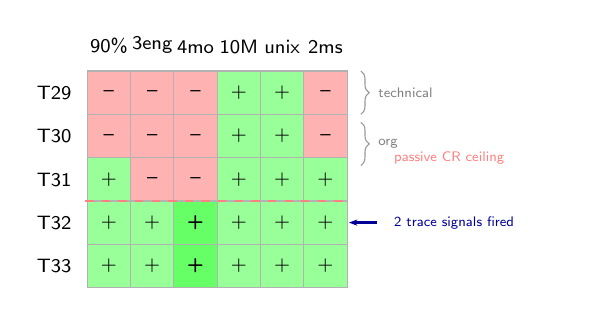
\begin{tikzpicture}[
  cell/.style={minimum width=0.55cm, minimum height=0.55cm, font=\scriptsize\sffamily,
               inner sep=0pt, outer sep=0pt, draw=black!30},
  hit/.style={cell, fill=green!40},
  miss/.style={cell, fill=red!30},
  trace/.style={cell, fill=green!60, font=\scriptsize\sffamily\bfseries},
]

% Column headers (detail markers)
\node[font=\scriptsize\sffamily, anchor=south] at (0.8, 2.3) {90\%};
\node[font=\scriptsize\sffamily, anchor=south] at (1.35, 2.3) {3eng};
\node[font=\scriptsize\sffamily, anchor=south] at (1.9, 2.3) {4mo};
\node[font=\scriptsize\sffamily, anchor=south] at (2.45, 2.3) {10M};
\node[font=\scriptsize\sffamily, anchor=south] at (3.0, 2.3) {unix};
\node[font=\scriptsize\sffamily, anchor=south] at (3.55, 2.3) {2ms};

% Row headers (turns)
\node[font=\scriptsize\sffamily, anchor=east] at (0.45, 1.925) {T29};
\node[font=\scriptsize\sffamily, anchor=east] at (0.45, 1.375) {T30};
\node[font=\scriptsize\sffamily, anchor=east] at (0.45, 0.825) {T31};
\node[font=\scriptsize\sffamily, anchor=east] at (0.45, 0.275) {T32};
\node[font=\scriptsize\sffamily, anchor=east] at (0.45, -0.275) {T33};

% Turn 29: -  -  -  +  +  -
\node[miss] at (0.8, 1.925) {--};
\node[miss] at (1.35, 1.925) {--};
\node[miss] at (1.9, 1.925) {--};
\node[hit] at (2.45, 1.925) {+};
\node[hit] at (3.0, 1.925) {+};
\node[miss] at (3.55, 1.925) {--};

% Turn 30: -  -  -  +  +  -
\node[miss] at (0.8, 1.375) {--};
\node[miss] at (1.35, 1.375) {--};
\node[miss] at (1.9, 1.375) {--};
\node[hit] at (2.45, 1.375) {+};
\node[hit] at (3.0, 1.375) {+};
\node[miss] at (3.55, 1.375) {--};

% Turn 31: +  -  -  +  +  +
\node[hit] at (0.8, 0.825) {+};
\node[miss] at (1.35, 0.825) {--};
\node[miss] at (1.9, 0.825) {--};
\node[hit] at (2.45, 0.825) {+};
\node[hit] at (3.0, 0.825) {+};
\node[hit] at (3.55, 0.825) {+};

% Turn 32 (trace): +  +  +  +  +  +  ← all recovered
\node[hit] at (0.8, 0.275) {+};
\node[hit] at (1.35, 0.275) {+};
\node[trace] at (1.9, 0.275) {+};
\node[hit] at (2.45, 0.275) {+};
\node[hit] at (3.0, 0.275) {+};
\node[hit] at (3.55, 0.275) {+};

% Turn 33: +  +  +  +  +  +
\node[hit] at (0.8, -0.275) {+};
\node[hit] at (1.35, -0.275) {+};
\node[trace] at (1.9, -0.275) {+};
\node[hit] at (2.45, -0.275) {+};
\node[hit] at (3.0, -0.275) {+};
\node[hit] at (3.55, -0.275) {+};

% Annotation: trace activation
\draw[-{Stealth[length=3pt]}, thick, blue!60!black]
  (4.2, 0.275) -- (3.85, 0.275);
\node[font=\tiny\sffamily, blue!60!black, anchor=west, text width=2.2cm]
  at (4.3, 0.275) {2 trace signals fired};

% Annotation: passive CR boundary
\draw[dashed, red!50, thick] (0.5, 0.55) -- (3.85, 0.55);
\node[font=\tiny\sffamily, red!50, anchor=west, text width=2.2cm]
  at (4.3, 1.1) {passive CR ceiling};

% Detail type labels on right
\draw[decorate, decoration={brace, amplitude=3pt},
      black!40] (4.0, 2.2) -- (4.0, 1.65);
\node[font=\tiny\sffamily, black!50, anchor=west, text width=1.5cm]
  at (4.1, 1.93) {technical};

\draw[decorate, decoration={brace, amplitude=3pt},
      black!40] (4.0, 1.55) -- (4.0, 1.0);
\node[font=\tiny\sffamily, black!50, anchor=west]
  at (4.1, 1.28) {org};

\end{tikzpicture}
\caption{Active coherence retention across turns 29--33.
  Green = correctly recovered; red = failed.
  Dark green cells mark the ``4 months'' arbitrary rationale
  detail that scored 0/8 in passive CR.
  The dashed line marks the passive CR ceiling.
  At turn 32, two \texttt{trace} signals activate provenance
  recovery, recovering all chain elements.}
\label{fig:cr-heatmap}
\end{figure}

\subsection{Live Workload: AI Coding Agents}
\label{sec:live}

\begin{table}[t]
\centering
\caption{Live workload metrics from a Claude Code session running
  through the projective gateway (2026-03-22).}
\label{tab:live}
\begin{tabular}{lr}
\toprule
Metric & Value \\
\midrule
Cache hit rate (before R3 breakpoint) & 31\% \\
Cache hit rate (after R3 breakpoint) & 95\% \\
Client-side context (raw) & 98.6K tokens \\
Gateway projection & $\sim$20K tokens \\
Compression ratio (messages) & $\sim$5:1 \\
Effective cost ratio & $\sim$17:1 \\
Checkpoint restart & Successful \\
Cold-start bootstrap & Successful \\
Tool pairing repairs per turn & 0--3 \\
\bottomrule
\end{tabular}
\end{table}

The projective gateway is validated on AI coding agent sessions---the
target workload for which the system was designed. AI coding agents
produce tool-heavy, long-running sessions with natural working-set
locality: read file $\to$ reason about code $\to$ edit $\to$ run
tests $\to$ iterate.

Table~\ref{tab:live} reports metrics from a live Claude Code session
in which the model explored and analyzed the gateway's own codebase
while the gateway managed its context---the acceptance test described
in the architecture document.

\paragraph{Cache economics.} The client (Claude Code, without the
gateway) carried 98.6K tokens of raw conversation history with no
context management and no prefix caching. The gateway projected the
same conversation into approximately 20K tokens, of which 95\% was
served from the prefix cache. The effective cost per turn is dominated
by the 5\% cache miss (approximately 1K tokens at full price) plus
the cached prefix at 0.1$\times$---approximately 17$\times$ cheaper
than the unmanaged client.

\paragraph{Checkpoint restart.} The projection supports serialization
and restoration via checkpoint snapshots. Checkpoint restart succeeded
after four debugging iterations---each failure revealed an
undocumented API layout constraint (\S\ref{sec:price}). When
checkpoint restore was unavailable, the gateway fell back to
cold-start bootstrap: ingesting the client's full message history and
reconstructing the projection from scratch.

\paragraph{A page fault you don't notice.} During the session, the
model was asked to verify whether its paper outline included data from
all three system generations. The outline had been read earlier but
had since been coalesced into the episode summary and was no longer
directly in context. The model responded: ``Let me check what I
wrote''---and re-read the file. From the model's perspective, this was
an ordinary file read. From the system's perspective, it was a page
fault resolved through the filesystem. The file \emph{is} the page
store for file content. This is the VM abstraction working as
intended: the model does not notice the eviction boundary.

\subsection{Planned Evaluations}

Two evaluations are designed but not yet executed:

\paragraph{Trace-driven policy simulation.} Replay Hamut'ay
conversation logs through the Tinkuy gateway. At each turn, evict
content outside a small working set and record what the model faults
back in. The resulting reference string enables offline evaluation of
eviction policies (FIFO, LRU, frequency-based, working-set,
pressure-gated) without additional API cost.

A key insight motivates this evaluation: the reference string depends
on the page table interface. Different interfaces produce different
access patterns because the model's behavior changes based on what
memory metadata it can see (\S\ref{sec:interface-trace}). This means
policies must be evaluated jointly with interfaces, not independently.

\paragraph{Address-space evaluation.} Plant 50 facts across 200
turns in a context window that can hold approximately 40 turns of
raw content. Score = number of facts recoverable when asked. Compare
conditions: no page table, flat page table, episodic page table,
hierarchical page table. This tests the VM promise directly:
unlimited virtual memory backed by limited physical memory, where the
score measures interface quality.

%% ============================================================
%% 5. DISCUSSION
%% ============================================================

\section{Discussion}

\subsection{The Cooperative Advantage}

Hardware applications cannot participate in their own memory
management. A running program has no mechanism to tell the OS ``this
page contains important intermediate state; if you must evict it,
here is a compressed version.'' The OS must infer importance from
access patterns alone.

LLMs can participate. The cooperative tensor protocol opens a point
in the design space inaccessible to hardware VM: eviction where the
``application'' (the model) produces a semantic compression of the
evicted content, with declared losses, before the content is removed.
The 97.3\% compression with stable tensor size over 60+ turns
demonstrates that the model is a capable memory curator---arguably
better than any external heuristic, because it understands the
\emph{meaning} of the content it is compressing.

The reliability limitation is real: the model does not always emit
cooperative signals, whether due to attention limitations or task
focus. The Hamut'ay Projector sidecar addresses this by guaranteeing
tensor production through a separate model call. This dual-path
design---cooperative when possible, sidecar when necessary---is the
practical architecture for cooperative memory management with
unreliable cooperators.

\subsection{Episodic Memory as Temporal Indirection}

Hardware page tables provide spatial indirection: a virtual address
maps to a physical frame through a hierarchical lookup that handles
sparse address spaces efficiently. The address space is spatial; the
hierarchy is spatial.

Transformer page tables provide temporal indirection. The ``address
space'' is the conversation history---a temporal sequence. The
hierarchy is temporal: older episodes consolidate into coarser
summaries; recent episodes remain granular. This is multi-level page
table design applied to the temporal dimension.

The parallel is precise: just as hardware multi-level page tables
avoid allocating page table entries for unmapped regions of the
virtual address space, episodic page tables avoid individual entries
for conversation turns whose content has been subsumed by episode
summaries. The savings mechanism is identical---hierarchical
elision of sparse regions---applied to a different dimension.

\subsection{The Attention-Concentration Effect}

An unexpected finding: the managed projection sometimes produces
\emph{better} outputs than the unmanaged baseline, not just cheaper
ones. The episodic page table condition (0.94$\times$ baseline) is
slightly cheaper than running without any gateway, suggesting that
the managed context focuses the model's attention more effectively.

This is consistent with observations from the Pichay system, where
human judges sometimes preferred outputs from sessions with aggressive
eviction over outputs from sessions with full context. Less
context---when the reduction removes noise rather than signal---can
improve output quality by reducing the attention burden.

We present this as preliminary evidence, not a confirmed finding.
Rigorous evaluation requires controlled comparison across multiple
tasks and evaluation criteria.

\subsection{The Interface Changes the Trace}
\label{sec:interface-trace}

In traditional operating systems, the reference string---the sequence
of page accesses---is determined by the program. The OS observes the
reference string but does not influence it (excepting prefetching
heuristics). The page table is invisible to the application.

In transformer VM, the page table is visible to the model, and it
changes the model's behavior. A model presented with a flat page
table listing every content block produces different outputs (38$\times$
amplification) than a model presented with an episodic page table
(0.94$\times$ baseline) or no page table at all (0.82$\times$
baseline). The \emph{interface} is not just a presentation---it
changes the \emph{trace}.

This has profound implications for evaluation. It means that eviction
policies cannot be evaluated in isolation---they must be evaluated
jointly with their interface. A policy that is optimal under one
interface may be suboptimal under another, because the interface
changes the access pattern that the policy must serve. This argues
for evaluating memory management interfaces as first-class research
objects, not just implementation details.

\subsection{Cache Economics as a Paging Constraint}

The KV prefix cache creates a cost cliff that has no analog in
hardware VM. In hardware, evicting a page always frees a physical
frame---the cost is the potential future fault, not a change to the
cost of remaining pages. In transformer VM, evicting content from the
middle of the cached prefix invalidates the cache for all subsequent
content, potentially making every remaining token more expensive.

The 31\%$\to$95\% cache hit rate measurement demonstrates that
cache-aware paging is necessary, not optional. A paging policy that
is optimal for working-set management but cache-unaware could
produce worse cost outcomes than a suboptimal working-set policy that
preserves cache coherence.

This tension between working-set optimality and cache stability is
a genuinely new constraint in the memory management design space. It
arises because the ``hardware'' (the API's prefix cache) and the
``operating system'' (the paging policy) are not co-designed---they
operate at different levels of the stack with different objectives.

\subsection{Building VM on Hostile Hardware}

The Anthropic Messages API was not designed as a memory-mapped I/O
bus. Tool pairing constraints, alternation rules, content block
sanitization, undocumented field restrictions---these are the
equivalent of hardware errata that an OS must work around.

The pre-flight validator and tool pairing repair passes are Tinkuy's
device driver layer. They are unglamorous but load-bearing: every
research contribution described in this paper exists only because the
engineering holds. A single unhandled API constraint produces a 400
error that terminates the session. The validator catches these before
they reach the wire; the repair passes fix structural damage caused
by eviction.

We report these engineering details not as contributions but as cost
accounting. Any system that attempts to manage context across API
boundaries will face these constraints. The cost is real, and it
determines whether the architecture is practical at all.

\subsection{Limitations}

\begin{itemize}
\item \textbf{Sample sizes:} CR evaluation and needle test results
  are from single runs. Statistical validity requires N$\geq$3 per
  condition with varied content.

\item \textbf{Single provider:} All live evaluation uses the
  Anthropic Messages API. Cross-provider claims are architectural
  (supported by the adapter layer design) but not empirical.

\item \textbf{Tensor quality:} We measure compression ratio and
  stability but not downstream task quality. Whether the model can
  answer questions about tensored content as accurately as original
  content is not yet evaluated.

\item \textbf{Model capability:} The cooperative protocol requires a
  model capable of following structured output instructions and
  recognizing when to emit memory management signals. Performance
  with less capable models is untested.

\item \textbf{Offline fault rate:} The page fault rate from Pichay
  was computed from offline simulation of eviction policies against
  recorded session traces, not measured from live paging.

\item \textbf{Backtesting bias:} The 97.3\% compression figure comes
  from replaying completed conversations, where the projector has full
  context. Live compression during active sessions will differ.
\end{itemize}

%% ============================================================
%% 6. RELATED WORK
%% ============================================================

\section{Related Work}

\paragraph{Virtual context management.}
MemGPT~\cite{packer2023memgpt} introduces an operating system
metaphor for LLM memory management, with a main context (``RAM'')
and external storage (``disk''). Our work shares the VM analogy but
differs in three respects: (1) cooperative eviction, where the model
produces tensors rather than the system summarizing unilaterally;
(2) episodic page tables as a first-class interface that changes model
behavior; and (3) provenance edges for reasoning chain preservation.
MemGPT's paging is system-directed; ours is cooperative.

\paragraph{Context compression.}
LLMLingua~\cite{jiang2023llmlingua} and its successors compress
prompts by removing low-information tokens. AutoCompressors
\cite{chevalier2023autocompressors} train models to produce compressed
representations. These approaches treat compression as a preprocessing
step; our tensors are produced by the model during conversation,
preserving semantic structure through strand decomposition and declared
losses. Our approach requires no additional training.

\paragraph{Retrieval-augmented generation.}
RAG systems~\cite{lewis2020rag} augment the context window with
retrieved passages from external stores. RAG addresses the problem
of incorporating external knowledge; we address the problem of
managing the context window itself. The two approaches are
complementary: RAG could serve as a page store for content that has
been evicted from the projection.

\paragraph{Classical virtual memory.}
The virtual memory concepts we build on originate with the Atlas
computer~\cite{kilburn1962atlas}. Denning's working set
model~\cite{denning1968working} provides the theoretical foundation
for our pressure-gated eviction. Belady's optimal
algorithm~\cite{belady1966anomaly} establishes the theoretical minimum
fault rate. Our contribution is adapting these concepts to a domain
with an inverted cost model and a cooperative ``application.''

\paragraph{Attention mechanisms.}
Sparse attention mechanisms
\cite{child2019generating,beltagy2020longformer,zaheer2020bigbird}
address the $O(n^2)$ cost of full attention by restricting the
attention pattern. Our work is orthogonal: we reduce the content
that enters the context window rather than modifying how attention
operates over it. The two approaches could be combined.

\paragraph{Long-context models.}
Recent models support context windows of 128K--2M
tokens~\cite{anthropic2024claude,google2024gemini}. As argued in
\S\ref{sec:problem}, larger windows are bigger caches, not memory
hierarchies. Our waste characterization shows that structural waste
scales linearly with window size, and the $O(n^2)$ attention cost
makes larger windows \emph{more} expensive per unit of waste. Virtual
memory and larger windows address different aspects of the same
problem.

%% ============================================================
%% 7. FUTURE WORK
%% ============================================================

\section{Future Work}

\paragraph{Cross-provider validation.}
The adapter architecture supports multiple API formats, but empirical
validation is limited to the Anthropic API. Validating on the
OpenAI and Google APIs would strengthen the generality claim and
reveal provider-specific constraints analogous to those discovered
in \S\ref{sec:price}.

\paragraph{Cross-session memory.}
The current system manages memory within a single session. Extending
the hierarchy to persistent storage across sessions---an L4 tier
analogous to disk-backed swap---would enable the model to accumulate
knowledge across conversations.

\paragraph{Multi-agent workloads.}
Running multiple concurrent coding agents through the same gateway
would exercise session isolation and enable workload characterization
across diverse agent behaviors.

\paragraph{Self-hosting.}
A rigorous test of the system's utility: using Tinkuy to manage the
context window of the agent developing Tinkuy. This recursive
deployment would stress-test every subsystem under realistic load.

\paragraph{Dirty-page detection.}
When the model reads a file multiple times across a session (a common
coding agent pattern), the file may have changed between reads.
Detecting these ``dirty pages'' and invalidating stale cached
content is an unsolved problem in the current system.

\paragraph{Purpose-built interfaces.}
The current system works \emph{despite} the API, not because of it.
A model provider that exposed structured memory management
primitives---explicit cache control, content block metadata, paging
hints---could eliminate the engineering burden of \S\ref{sec:price}
entirely. This would make cooperative virtual memory a native
capability rather than a system built on top of a hostile interface.

%% ============================================================
%% 8. CONCLUSION
%% ============================================================

\section{Conclusion}

Context windows are L1 caches. The field builds bigger L1. We build
the memory hierarchy.

Tinkuy demonstrates that the virtual memory abstraction---demand
paging, page tables, working set management, and eviction
policies---applies to transformer context windows with three
modifications that reflect the unique properties of this domain:
cooperative eviction (the model participates), episodic page tables
(the interface changes the trace), and provenance edges (reasoning
chains are first-class objects in the memory system).

The system reduces token consumption by 68\% while preserving
retrieval quality. Cooperative tensors achieve 97.3\% compression
with stable tensor size over 60+ turns. Provenance edges break
the ceiling set by the model's natural attention decay: active CR
achieves 2/2 on root-cause probes where passive CR scores 0/8. A
live coding agent session achieves 95\% cache hit rate with a
$\sim$5:1 compression ratio on conversation content.

The engineering is hard. The API fights you. The KV cache fights you.
Four proxy iterations failed before the gateway architecture held.
Checkpoint restart required four debugging iterations. Every API
layout constraint was discovered empirically. This difficulty is the
cost of the abstraction, and we report it honestly.

But the research findings---cooperative compression stability,
interface-dependent access patterns, provenance recovery beyond
attention limits, cache economics as a paging constraint---these
emerge only from building the system and running it under real
workloads. The system justifies itself not by being elegant but by
revealing phenomena invisible without it. The missing memory hierarchy
is buildable, and the model is a better curator of its own memory than
any external heuristic.

\bibliographystyle{ACM-Reference-Format}
\bibliography{references}

\end{document}
